\documentclass[aps,letterpaper,11pt]{revtex4}
\usepackage{graphicx} % For images
\usepackage{float}    % For tables and other floats
\usepackage{verbatim} % For comments and other
\usepackage{amssymb}  % For more math
\usepackage{fullpage} % Set margins and place page numbers at bottom center
\usepackage{listings} % For source code
\usepackage[usenames,dvipsnames]{color} % For colors and names
\usepackage[pdftex]{hyperref}           % For hyperlinks and indexing the PDF
\usepackage{pdfpages}
\usepackage{subfig}
\usepackage{listings}
\usepackage[usenames,dvipsnames,svgnames,table]{xcolor}
\usepackage{color}
\usepackage{textcomp}
\usepackage[utf8]{inputenc}
% Custom colors
\definecolor{deepblue}{rgb}{0,0,0.5}
\definecolor{deepred}{rgb}{0.6,0,0}
\definecolor{deepgreen}{rgb}{0,0.5,0}

 \lstset{
  tabsize=4,
  language=C++,
  captionpos=b,
  tabsize=3,
  numberstyle=\tiny,
  numbersep=5pt,
  breaklines=true,
  showstringspaces=false,
  basicstyle=\footnotesize,
%  identifierstyle=\color{magenta},
  keywordstyle=\color[rgb]{0,0,1},
  commentstyle=\color{deepgreen},
  stringstyle=\color{deepred}
  }
  
\hypersetup{ % play with the different link colors here
    colorlinks,
    citecolor=black,
    filecolor=black,
    linkcolor=black,
    urlcolor=blue % set to black to prevent printing blue links
}

\newcommand{\labno}{Software Engineering Project}
\newcommand{\labtitle}{User's Manual}
\newcommand{\authorname}{Group members:\\Antoine Merlet\\Gülnur Ungan\\Mladen Rakic\\Marcio Aloisio Bezerra Cavalcanti Rockenbach}
\newcommand{\professor}{Dr. Yohan Fougerolle, Dr. Cansen Jiang, Dr. David Strubel}

   

\begin{document}  
\begin{titlepage}
\begin{center}
{\LARGE \textsc{\labno:} \\ \vspace{4pt}}
{\Large \textsc{\labtitle} \\ \vspace{4pt}} 
\rule[13pt]{\textwidth}{1pt} \\ \vspace{150pt}
\begin{figure}[!htb]
  
\includegraphics[scale=1.0]{logo.jpg}
\end{figure}
{\large  \authorname \\ \vspace{10pt}
Professor: \professor \\ \vspace{10pt}
\today}
\end{center}




\end{titlepage}% END TITLE PAGE %%%%%%%%%%%%%%%%%%%%%%%%%%%%%%%%%%
\newpage

\section{Main Window}

\begin{figure}[H]
	\centering
	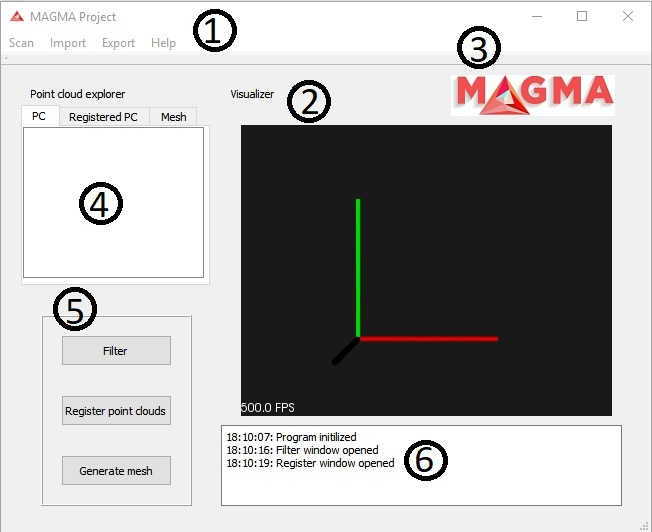
\includegraphics[width=15cm]{Gui_main_1.jpg}
	\caption{GUI main window design}
	\label{fig: GlobalDesignNumbers}    
\end{figure}

The GUI Main Window is organized as follow:

\begin{enumerate}
  \item \textbf{Upper Tools}: Allows the user to have access to the main tools of the program: New Scan, Import and Export Point Clouds and Help. They can be divided into subsections.
\begin{enumerate}
  \item \textbf{Scan}: Scan section includes:
\begin{enumerate}
  \item \textbf{New scan}: To start a new scan to capture point clouds from the Kinect.
\end{enumerate}
  \item \textbf{Import}: Import section includes:
\begin{enumerate}
  \item \textbf{Import point clouds}: Imports raw point clouds.
  \item \textbf{Import registered PC}: Imports registered point clouds.
\end{enumerate}
  \item \textbf{Export}: This section includes:
\begin{enumerate}
  \item \textbf{Export point clouds}: Saves raw point clouds into files.
 \item \textbf{Export registered PC}: Saves registered point clouds into files.
\end{enumerate}
  \item \textbf{Help}: To find solution of problems.
\begin{enumerate}
  \item \textbf{User manual}: Instructions for the users
 \item \textbf{About}: Information about the project and the developers
\end{enumerate}
\end{enumerate}

  \item \textbf{Visualizer}: Displays raw point clouds, registered point clouds and mesh
  \item\textbf{MAGMA Logo}: Project logo.
  \item \textbf{Point Cloud Explorer}
\begin{enumerate}
  \item \textbf{PC}:  Displays loaded raw point clouds in a list. The user can check or uncheck each item to display it in the visualizer.
 \item \textbf{Register PC}: Displays registered point clouds in a list. The user can check or uncheck each item to display it in the visualizer.
 \item \textbf{Mesh}: Displays meshes in a list. The user can check or uncheck each item to display it in the visualizer.
\end{enumerate}
 \item \textbf{Register Frame}:
\begin{enumerate}
  \item \textbf{Filter}: Opens filter window to allow the user to perform filter operations on the selected point clouds in the point cloud explorer.
 \item \textbf{Register Point Clouds}: Opens register window to allow the user to perform registering operations on the selected point clouds in the point cloud explorer.
 \item \textbf{Generate Mesh}: Generates mesh from registered point clouds.
\end{enumerate}
 \item \textbf{Logger Display}: Displays logger messages (generated by the program during execution)
\end{enumerate}



\section{Filtering}

\begin{figure}[H]
	\centering
	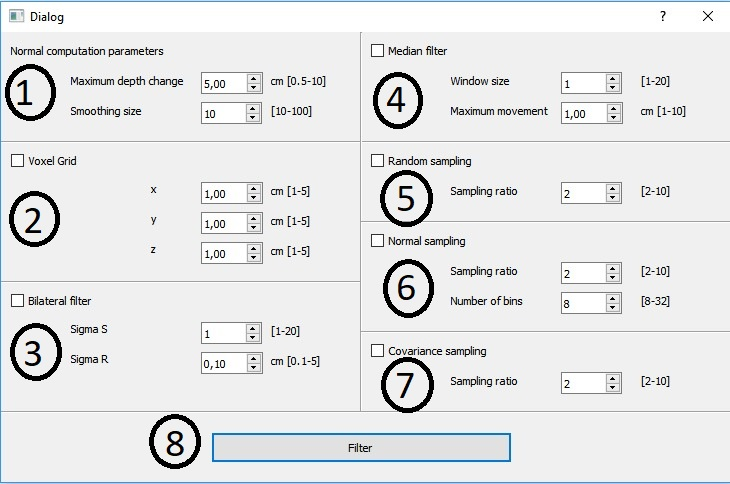
\includegraphics[width=15cm]{Gui_filter_1.jpg}
	\caption{GUI filtering window design}
	\label{fig: GlobalDesignNumbers}    
\end{figure}

This window display the different filters that can be applied to the point clouds. Each of these filters can be checked or not according to the user (if the user wants to use them or not). All of them have parameters that can be altered by the user and then applied. The Filtering Window is organized as follows:

\begin{enumerate}
  \item \textbf{Normal computation parameters}:It is used for input point cloud in the space of normal directions computed at every point.
\begin{enumerate}
  \item \textbf{Maximum depth change}: The depth change threshold for computing object borders based on depth changes.
  \item \textbf{Smoothing size}: The factor which influences the size of the area used to smooth normals .
\end{enumerate}
 \item \textbf{Voxel Grid}: It is used to downsample the given point cloud.
\begin{enumerate}
 \item \textbf{x}: Size of filter.
 \item \textbf{y}: Size of filter.
 \item \textbf{z}: Size of filter.
\end{enumerate}
 \item \textbf{Bilateral Filter}: It is used for smoothing depth information in organized point clouds.
\begin{enumerate}
 \item \textbf{Sigma S}: The size of the Gaussian bilateral filter window to use.
 \item \textbf{Sigma R}: The standard deviation of the Gaussian for the intensity difference.
\end{enumerate}
 \item \textbf{Median Filter}: It is implementation of the median filter.
\begin{enumerate}
 \item \textbf{Window Size}: Setting the window size of the filter.
 \item \textbf{Maximum Movement}: Maximum value a dexel is allowed to move during filtering.
\end{enumerate}
 \item \textbf{Random Sampling}: Random sampling with uniform probability.
\begin{enumerate}
 \item \textbf{Sampling Ratio}: The ratio of sample size to total size.
\end{enumerate}
 \item \textbf{Normal Sampling}: 
\begin{enumerate}
 \item \textbf{Sampling Ratio}: The ratio of sample size to total size.
 \item \textbf{Number of Bins}: Number of bins that is used.
\end{enumerate}
 \item \textbf{Covariance Sampling}: It selects the points such that the resulting cloud is as stable as possible for being registered (against a copy of itself) with ICP.
\begin{enumerate}
 \item \textbf{Sampling Ratio}: The ratio of sample size to total size.
\end{enumerate}
 \item \textbf{Filter}: It is used to apply selected filter.
\end{enumerate}


\section{Registration}

\begin{figure}[H]
	\centering
	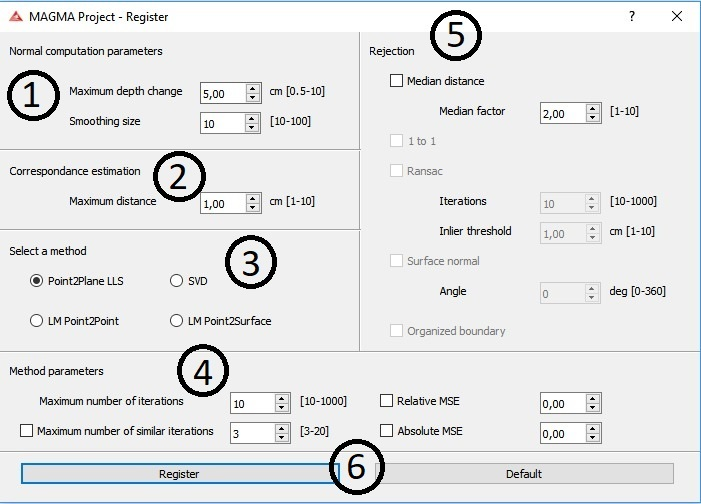
\includegraphics[width=15cm]{Gui_regist_1.jpg}
	\caption{GUI registration window design}
	\label{fig: GlobalDesignNumbers}    
\end{figure}

This window display the different registration methods that can be applied to the point clouds. Each of these methods can be checked or not according to the user (if the user wants to use them or not). All of them have parameters that can be altered by the user and then applied. The Registration Window is organized as follows:

\begin{enumerate}
  \item \textbf{Normal computation parameters}:
\begin{enumerate}
  \item \textbf{Maximum depth change}:  The depth change threshold for computing object borders based on depth changes.
  \item \textbf{Smoothing size}: The factor which influences the size of the area used to smooth normals .
\end{enumerate}
 \item \textbf{Correspondence estimation}:
\begin{enumerate}
 \item \textbf{Maximum distance}:
\end{enumerate}
 \item \textbf{Select a method}: One method of 4 different algorithms is chosen as follows:
\begin{enumerate}
 \item \textbf{Point2Plane LLS}: Point to plane linear least square method.
 \item \textbf{SVD}: Singular value decomposition method.
 \item \textbf{LM Point2Point}: Levenberg Marquardt point to point method.
\item \textbf{LM Point2Surface}: Levenberg Marquardt point to surface method.
\end{enumerate}
 \item \textbf{Method Parameters}: For selected method, the below parameters are tuned.
\begin{enumerate}
 \item \textbf{Maximum number of iterations}: Number of maximum iteration is chosen.
 \item \textbf{Maximum number of similar iterations}: Number of similar iteration is chosen.
 \item \textbf{Relative MSE}: Relative mean square error.
 \item \textbf{Absolute MSE}: Absolute mean square error.
\end{enumerate}
 \item \textbf{Rejection}: To reject, following parameters are set:
\begin{enumerate}
 \item \textbf{Median distance}: Median distance between correspondences.
\begin{enumerate}
 \item \textbf{Median factor}: Median factor between correspondences
\end{enumerate}
 \item \textbf{1 to 1}: 
 \item \textbf{Ransac}: Random sample consensus (RANSAC) is an iterative method to estimate parameters of a mathematical model from a set of observed data that contains outliers, when outliers are to be accorded no influence on the values of the estimates.
\begin{enumerate}
 \item \textbf{Iterations}: Number of iterations.
 \item \textbf{Inlier threshold}: Ransac inlier threshold value. 
\end{enumerate}
 \item \textbf{Surface normal}:To a surface at a point P is a vector that is perpendicular to the tangent plane to that surface at P. 
\begin{enumerate}
 \item \textbf{Angle}: Angle of  surface normal. (In degrees)
\end{enumerate}
 \item \textbf{Organized boundary}: Boundaries are chosen.
\end{enumerate}
 \item \textbf{Register and Default}: When you click register, program works according to your tuned parameters. Default option gives the result according to default values.
\end{enumerate}


\end{document} % DONE WITH DOCUMENT!